% Provenance (never printed): see sources/outline_sources.md (Year 3: rift
% models, normal-fault systems, metamorphic core complexes, strike-slip
% systems). Brief: sources/book5/BRIEFS.md, ch. 9. Curves from
% figdata/bachelor-3/domino_extension.py and rollover.py. Exercise and problem
% values in the Book 5 scratch calculator calc/ch09.py.
\chapter{Tectônica extensional e transcorrente}\label{ch:b3:extension-strike-slip}

Entre a Sierra Nevada e o Planalto do Colorado, serras e bacias
se alternam como os sulcos de um campo, cada serra um bloco de crosta inclinado
ao longo de uma falha normal. No núcleo de algumas dessas serras, rochas que
foram soterradas entre 23 e \qty{30}{km} de profundidade, a temperaturas entre 500 e \qty{650}{\celsius}, hoje afloram na
superfície, sob uma única falha que mergulha apenas alguns graus. Um continente pode
ser distendido por um fator de dois ou mais, e rasgado lateralmente ao longo de falhas
que se curvam, se escalonam e abrem bacias tão profundas quanto \qty{10}{km}. Este capítulo constrói
a geometria da extensão e do falhamento transcorrente, as poucas regras que
as regem e as evidências que os sistemas reais deixam.
% ledger: cooper10:snake-range, mcq05:basin-range, tb93:dead-sea-basin

\begin{recall}
Falhas normais, transcorrentes e transformantes, o semigráben e o rifte continental
estão no volume do primeiro ano, nos capítulos sobre riftes e sobre falhas, dobras
e tramas, com a teoria de Anderson: com $\sigma_1$ vertical, as falhas normais
mergulham $\ang{45} + \phi/2$, cerca de \ang{60}; com $\sigma_2$ vertical, as falhas transcorrentes
têm direção a $\ang{45} - \phi/2$ de $\sigma_1$. A lei de Byerlee sobre o atrito das rochas,
$\tau = 0.85\,\sigma_n$ abaixo de \qty{200}{MPa} e $\tau =
\qty{50}{MPa} + 0.6\,\sigma_n$ acima, está no capítulo sobre tensão, deformação e
reologia. O modelo de estiramento, em que a litosfera é adelgaçada uniformemente
por um fator $\beta$, e a bacia de rifte encontram-se no volume do segundo ano, no seu
capítulo que compara bacias sedimentares. \omterm{def:b3:deformation-mechanisms:shear-zone}{Zonas de cisalhamento} e milonitos estão no
\cref{ch:b3:deformation-mechanisms}; a profundidade até o descolamento a partir de uma área em excesso,
área, $A = Sh$, no \cref{ch:b3:structural-analysis}.
\end{recall}
% ledger: byerlee:1975

\section{Dois modelos de rifte}\label{sec:b3:extension-strike-slip:models}

O modelo de estiramento do volume do segundo ano adelgaça toda a litosfera pelo
mesmo fator sob o mesmo lugar: crosta e manto adelgaçam-se juntos,
de forma simétrica, por cisalhamento puro. Muitas margens de rifte não são simétricas: um lado
é uma região larga de blocos inclinados, o outro um talude estreito e íngreme, e o
adelgaçamento do manto situa-se ao lado, e não sob, o adelgaçamento da crosta.

\begin{definition}[Modelo de rifte por cisalhamento simples]\label{def:b3:extension-strike-slip:rift-models}
No \emph{modelo de rifte por cisalhamento simples}\index{modelo de rifte por cisalhamento simples} a
litosfera é distendida ao longo de uma \omterm{def:b3:deformation-mechanisms:shear-zone}{zona de cisalhamento} de baixo ângulo que a atravessa
da superfície até a base. A placa acima da \omterm{def:b3:deformation-mechanisms:shear-zone}{zona de cisalhamento}, a placa superior,
perde sua parte inferior; a placa abaixo, a placa inferior, é puxada para fora
de sob ela. O adelgaçamento da crosta e o adelgaçamento do manto estão
deslocados lateralmente, e as duas margens conjugadas que se formam quando o continente
se rompe são assimétricas.
\end{definition}

Riftes reais misturam os dois: falhamento frágil na crosta superior, adelgaçamento dúctil
abaixo, e um manto que pode adelgaçar-se em uma região mais larga ou mais estreita que a
crosta (estiramento dependente da profundidade). Onde o manto quente sobe sob o
rifte, ou sob um de seus flancos no caso de cisalhamento simples, a flutuabilidade eleva os
ombros do rifte, que se erguem como montanhas acima do assoalho da bacia.

\begin{omfigure}
\begin{tikzpicture}[scale=0.95, >=stealth]
% (a) pure shear
\begin{scope}
\fill[omLithBasalt!40] (0,-3.2) rectangle (6.6,-1.3);
\fill[omLithGranite!50] (0,0) -- (2.2,0) -- (2.5,-0.35) -- (4.1,-0.35) -- (4.4,0) -- (6.6,0) -- (6.6,-1.3)
  -- (4.4,-1.3) -- (3.3,-0.95) -- (2.2,-1.3) -- (0,-1.3) -- cycle;
\fill[omLithBasalt!40] (2.2,-1.3) -- (3.3,-0.95) -- (4.4,-1.3) -- cycle;
\fill[orange!25] (0,-3.2) -- (1.8,-3.2) -- (3.3,-2.1) -- (4.8,-3.2) -- (6.6,-3.2) -- (6.6,-3.7) -- (0,-3.7) -- cycle;
\draw (0,0) -- (2.2,0) -- (2.5,-0.35) -- (4.1,-0.35) -- (4.4,0) -- (6.6,0);
\draw (0,-1.3) -- (2.2,-1.3) -- (3.3,-0.95) -- (4.4,-1.3) -- (6.6,-1.3);
\draw (0,-3.2) -- (1.8,-3.2) -- (3.3,-2.1) -- (4.8,-3.2) -- (6.6,-3.2);
\draw[thick] (2.2,0) -- (2.75,-0.85); \draw[thick] (4.4,0) -- (3.85,-0.85);
\node[font=\scriptsize] at (0.7,-0.65) {crosta};
\node[font=\scriptsize, align=center] at (0.9,-2.25) {manto\\ litosfera};
\node[font=\scriptsize] at (1.2,-3.48) {astenosfera};
\draw[<-] (-0.1,0.25) -- (0.6,0.25); \draw[->] (6.0,0.25) -- (6.7,0.25);
\node[font=\small] at (3.3,-4.2) {(a) cisalhamento puro};
\end{scope}
% (b) simple shear: crust thinned near the breakaway (left), mantle beneath the upper plate (right)
\begin{scope}[xshift=7.4cm]
\fill[omLithBasalt!40] (0,-3.2) rectangle (6.6,-1.3);
\fill[omLithGranite!50] (0,0) -- (0.9,0) -- (1.2,-0.3) -- (2.2,-0.3) -- (2.5,0) -- (4.0,0)
  .. controls (4.6,0.18) and (5.2,0.18) .. (5.8,0) -- (6.6,0) -- (6.6,-1.3)
  -- (2.9,-1.3) -- (2.0,-0.7) -- (1.2,-1.3) -- (0,-1.3) -- cycle;
\fill[omLithBasalt!40] (1.2,-1.3) -- (2.0,-0.7) -- (2.9,-1.3) -- cycle;
\fill[orange!25] (0,-3.2) -- (3.4,-3.2) -- (4.8,-2.1) -- (6.0,-3.2) -- (6.6,-3.2) -- (6.6,-3.7) -- (0,-3.7) -- cycle;
\draw (0,0) -- (0.9,0) -- (1.2,-0.3) -- (2.2,-0.3) -- (2.5,0) -- (4.0,0)
  .. controls (4.6,0.18) and (5.2,0.18) .. (5.8,0) -- (6.6,0);
\draw (0,-1.3) -- (1.2,-1.3) -- (2.0,-0.7) -- (2.9,-1.3) -- (6.6,-1.3);
\draw (0,-3.2) -- (3.4,-3.2) -- (4.8,-2.1) -- (6.0,-3.2) -- (6.6,-3.2);
\draw[omThm, very thick] (0.9,0) .. controls (2.4,-0.9) and (3.9,-1.8) .. (5.4,-3.2);
\node[font=\scriptsize, align=center] at (5.0,-0.6) {placa superior};
\node[font=\scriptsize, align=center] at (1.3,-2.3) {placa inferior};
\node[omThm, font=\scriptsize, align=center] at (3.0,-2.15) {zona\\ de cisalhamento};
\node[font=\scriptsize, align=center] at (4.9,0.42) {flanco soerguido};
\draw[<-] (-0.1,0.25) -- (0.6,0.25); \draw[->] (6.0,0.25) -- (6.7,0.25);
\node[font=\small] at (3.3,-4.2) {(b) cisalhamento simples};
\end{scope}
\end{tikzpicture}

\par\smallskip{\small Dois modelos extremos de rifte (fora de escala). (a) Cisalhamento
puro: a crosta e o manto litosférico adelgaçam-se juntos sob o rifte, com
falhas normais dos dois lados. (b) Cisalhamento simples: uma \omterm{def:b3:deformation-mechanisms:shear-zone}{zona de cisalhamento} de baixo ângulo atravessa
a litosfera; a crosta adelgaça-se perto de seu traço na superfície, o manto sob
o lado oposto, sob a placa superior, de modo que o rifte é assimétrico e seu
flanco acima do manto adelgaçado é soerguido.}\label{fig:b3:extension-strike-slip:models}
\end{omfigure}

\section{Sistemas de falhas normais}\label{sec:b3:extension-strike-slip:faults}

\begin{definition}[Falhamento em dominó]\label{def:b3:extension-strike-slip:domino}
No \emph{falhamento em dominó}\index{falhamento em dominó} um conjunto de falhas normais planares
paralelas corta a crosta superior em blocos rígidos que, à medida que a região
se distende, rotacionam juntos como uma fileira de livros caindo: as falhas tornam-se
menos íngremes e os estratos, inicialmente horizontais, inclinam-se no sentido oposto.
\end{definition}

\begin{theorem}[Extensão por dominós]\label{thm:b3:extension-strike-slip:domino}
Suponha-se que blocos rígidos, limitados por falhas planares paralelas que inicialmente mergulhavam
$\theta_0$ girem até que as falhas mergulhem $\theta$. Os estratos passam então a mergulhar $\theta_0
- \theta$, afastando-se das falhas, e a região foi distendida pelo
fator
\[
  \beta = \frac{\sin\theta_0}{\sin\theta} .
\]
\end{theorem}

\begin{proof}
Os blocos são rígidos, portanto a distância perpendicular $d$ entre duas
falhas vizinhas não muda. Ao longo de uma linha horizontal, dois planos paralelos
que mergulham $\theta$ e distam $d$ entre si cortam um segmento de comprimento $d/\sin
\theta$; a largura da região varia proporcionalmente ao comprimento desse segmento, de
$d/\sin\theta_0$ para $d/\sin\theta$. Os blocos giram pelo ângulo em que as falhas se achataram,
$\theta_0 - \theta$, e os estratos, inicialmente horizontais,
giram junto com eles.
\end{proof}

A rotação, sozinha, produz uma distensão modesta: falhas que começam em \ang{60} e
achatam-se até \ang{30} distendem a região por um fator $\beta = 1.73$. Elas não podem girar
para sempre: uma falha torna-se mais difícil de deslizar à medida que se achata, porque o
$\sigma_1$ vertical pressiona-a mais e a cisalha menos.

\begin{proposition}[Travamento por atrito de uma falha normal]\label{prop:b3:extension-strike-slip:lockup}
Suponha-se que uma falha sem coesão, de coeficiente de atrito $\mu$, forme o ângulo
$t$ com $\sigma_1$, todas as tensões efetivas. Ela desliza quando a razão entre as
tensões principais atinge
\[
  \frac{\sigma_1}{\sigma_3} = \frac{1 + \mu\cot t}{1 - \mu\tan t} ,
\]
que é mínima, $(\sqrt{1 + \mu^2} + \mu)^2$, em $\tan2t = 1/\mu$, e
infinita em $\tan t = 1/\mu$. Com $\sigma_1$ vertical, o mergulho da falha é
$\ang{90} - t$: uma falha normal com mergulho menor que $\arctan\mu$ não pode deslizar de
modo algum.
\end{proposition}

\begin{proof}
Escreve-se $m = (\sigma_1 + \sigma_3)/2$ e $s = (\sigma_1 - \sigma_3)/2$. No
plano, $\sigma_n = \sigma_1\sin^2t + \sigma_3\cos^2t = m - s\cos2t$ e
$\tau = (\sigma_1 - \sigma_3)\sin t\cos t = s\sin2t$. O deslizamento exige $\tau =
\mu\sigma_n$; dividindo por $\sigma_3\sin t\cos t$ e agrupando $\sigma_1$
obtém-se a razão, cujo denominador se anula em $\tan t = 1/\mu$. Na outra
forma, a condição lê-se $s(\sin2t + \mu\cos2t) = \mu m$. O colchete é no
máximo $\sqrt{1 + \mu^2}$, atingido em $\tan2t = 1/\mu$, onde o deslizamento exige o
menor $s/m = \mu/\sqrt{1 + \mu^2}$; então $\sigma_1/\sigma_3 = (m + s)/(m - s) =
(\sqrt{1 + \mu^2} + \mu)/(\sqrt{1 + \mu^2} - \mu) = (\sqrt{1 + \mu^2} +
\mu)^2$, pois o produto dos dois últimos colchetes é 1.
\end{proof}

Com o $\mu = 0.6$ de Byerlee, a falha normal mais bem orientada mergulha \ang{60.5} e
desliza quando $\sigma_1 = 3.12\,\sigma_3$; uma falha a \ang{45} exige $4.0$, e
nenhuma com mergulho menor que \ang{31} desliza; com $\mu = 0.85$ o mergulho de travamento é
\ang{40}. A figura abaixo mostra os dois resultados. Quando um conjunto de dominós se aproxima
do travamento, um novo conjunto de falhas íngremes corta o antigo: regiões muito distendidas
exibem várias gerações de falhas.

\begin{omfigure}
\begin{tikzpicture}
\begin{groupplot}[group style={group size=2 by 1, horizontal sep=1.6cm},
  omrecord, width=0.47\linewidth, height=0.42\linewidth, title style={font=\small},
  legend style={font=\scriptsize, legend cell align=left}]
\nextgroupplot[title={(a) distensão por dominós rígidos}, xlabel={mergulho atual da falha $\theta$ (\unit{\degree})},
  ylabel={fator de distensão $\beta$}, xmin=10, xmax=70, ymin=1, ymax=4,
  legend style={at={(0.97,0.97)}, anchor=north east}]
% computed in figdata/bachelor-3/domino_extension.py
\addplot[omDef, thick] table[x=dip, y=b70] {figdata/out/bachelor-3-domino_extension-beta.dat};
\addlegendentry{$\theta_0 = \ang{70}$}
\addplot[red!70!black, thick, densely dashed] table[x=dip, y=b60] {figdata/out/bachelor-3-domino_extension-beta.dat};
\addlegendentry{$\theta_0 = \ang{60}$}
\addplot[black, thick, densely dotted] table[x=dip, y=b45] {figdata/out/bachelor-3-domino_extension-beta.dat};
\addlegendentry{$\theta_0 = \ang{45}$}
\nextgroupplot[title={(b) razão de tensões necessária para o deslizamento}, xlabel={mergulho da falha (\unit{\degree})},
  ylabel={$\sigma_1/\sigma_3$}, xmin=20, xmax=90, ymode=log, ymin=1, ymax=40,
  log ticks with fixed point, ytick={1,2,5,10,20,40},
  legend style={at={(0.97,0.97)}, anchor=north east}]
\addplot[omDef, thick] table[x=dip, y=r060] {figdata/out/bachelor-3-domino_extension-lockup.dat};
\addlegendentry{$\mu = 0.6$}
\addplot[red!70!black, thick, densely dashed] table[x=dip, y=r085] {figdata/out/bachelor-3-domino_extension-lockup.dat};
\addlegendentry{$\mu = 0.85$}
\end{groupplot}
\end{tikzpicture}

\par\smallskip{\small (a) Fator de distensão de um domínio de dominós rígidos conforme
suas falhas giram do mergulho inicial $\theta_0$ até $\theta$. (b) Razão entre as
tensões principais efetivas necessárias para deslizar uma falha normal de determinado mergulho
sob um $\sigma_1$ vertical, para os dois coeficientes de atrito de Byerlee: mínima
perto de \ang{60} e \ang{65}, e infinita nos mergulhos de travamento \ang{31} e
\ang{40}.}\label{fig:b3:extension-strike-slip:domino}
\end{omfigure}

Muitas falhas normais grandes são curvas, íngremes na superfície e achatam-se em
profundidade até uma falha ou \omterm{def:b3:deformation-mechanisms:shear-zone}{zona de cisalhamento} quase horizontal.

\begin{definition}[Falha de descolamento, falha lístrica, anticlinal de rollover]\label{def:b3:extension-strike-slip:detachment}
Uma \emph{falha de descolamento}\index{falha de descolamento} é uma falha normal de baixo
ângulo ou \omterm{def:b3:deformation-mechanisms:shear-zone}{zona de cisalhamento} de grande deslocamento, de quilômetros a dezenas de quilômetros, que
separa uma placa superior distendida de uma placa inferior deformada de maneira diferente. Uma
\emph{falha lístrica}\index{falha lístrica} é uma falha normal cujo mergulho
diminui com a profundidade, sendo seu perfil côncavo para cima. Quando o bloco superior de
uma falha lístrica desce e se afasta, ela se curva para permanecer em contato com a
falha: seus estratos inclinam-se em direção à falha, em uma dobra ampla, o
\emph{anticlinal de rollover}\index{anticlinal de rollover}.
\end{definition}

\begin{method}[Construção de afastamento horizontal constante]\label{met:b3:extension-strike-slip:heave}
Para desenhar o bloco superior de uma \omterm{def:b3:extension-strike-slip:detachment}{falha lístrica} após um deslocamento horizontal
$H$, o afastamento horizontal, em uma seção paralela ao deslizamento:
\begin{enumerate}
  \item Divide-se o bloco superior em colunas verticais. Desloca-se cada coluna
        lateralmente em $H$, para longe do bloco inferior.
  \item Rebaixa-se cada coluna pelo desnível da falha sob ela: uma coluna que
        começou onde a falha está na profundidade $f(x)$ e termina onde ela está
        em $f(x + H)$, desce $f(x + H) - f(x)$, o que traz sua base
        de volta sobre a falha.
  \item O espaço deixado entre o bloco inferior e o bloco superior deslocado é o
        semigráben, preenchido à medida que se abre por sedimentos que se espessam em direção à
        falha.
\end{enumerate}
Lido de trás para frente, a construção restaura a seção e prevê a forma
da falha a partir da forma do rollover.
\end{method}

A área abaixo do nível original de um estrato, contada a partir da falha, é
a área do \cref{ch:b3:structural-analysis} com o sinal trocado: $A =
H(D - z_0)$ para um estrato situado inicialmente à profundidade $z_0$ acima de uma \omterm{def:b3:extension-strike-slip:detachment}{falha de descolamento} à
profundidade $D$, já que a rocha sob o estrato mantém sua área enquanto seu comprimento aumenta
em $H$. Medindo-se $A$ e $H$ em uma seção sísmica, obtém-se a profundidade da
\omterm{def:b3:extension-strike-slip:detachment}{falha de descolamento}. A figura abaixo ilustra a construção.

\begin{omfigure}
\begin{tikzpicture}
\begin{axis}[width=0.9\linewidth, height=0.36\linewidth, omsection,
  xmin=-2, xmax=24, ymin=0, ymax=6, y dir=reverse,
  xlabel={distância (\unit{km})}, ylabel={profundidade (\unit{km})},
  legend style={font=\scriptsize, legend cell align=left, at={(0.98,0.27)}, anchor=south east}]
% computed in figdata/bachelor-3/rollover.py (heave 2 km, detachment at 5 km)
\addplot[name path=fault, black, very thick] table[x=x, y=z] {figdata/out/bachelor-3-rollover-fault.dat};
\addlegendentry{falha lístrica}
\addplot[name path=top, omDef, thick] table[x=x, y=z] {figdata/out/bachelor-3-rollover-top.dat};
\addlegendentry{topo do bloco superior}
\addplot[omDef, thick, densely dashed] table[x=x, y=z] {figdata/out/bachelor-3-rollover-bed.dat};
\addlegendentry{um estrato inicialmente a \qty{2}{km}}
\addplot[gray, dashed, forget plot] coordinates {(-2,0) (24,0)};
\addplot[gray, dashed, forget plot] coordinates {(-2,5) (24,5)};
\node[font=\scriptsize, anchor=west] at (axis cs:15,5.35) {falha de descolamento};
\node[font=\scriptsize] at (axis cs:3.9,0.45) {semigráben};
\node[font=\scriptsize] at (axis cs:-1,1.5) {bloco inferior};
\node[font=\scriptsize] at (axis cs:9.5,1.15) {rollover};
\end{axis}
\end{tikzpicture}

\par\smallskip{\small \omterm{def:b3:extension-strike-slip:detachment}{Falha lístrica} com mergulho de \ang{60} na superfície e
achatando-se em uma \omterm{def:b3:extension-strike-slip:detachment}{falha de descolamento} a \qty{5}{km}, após um afastamento horizontal de \qty{2}{km}
traçado pela construção de afastamento constante. O topo do bloco superior e um
estrato mais profundo afundam em direção à falha, formando um rollover; a área abaixo do
topo original, \qty{10}{km^2}, é o afastamento horizontal vezes a profundidade da \omterm{def:b3:extension-strike-slip:detachment}{falha de descolamento}, e abaixo
do estrato mais profundo \qty{6}{km^2}, o afastamento horizontal vezes sua altura acima dele.}\label{fig:b3:extension-strike-slip:rollover}
\end{omfigure}

Falhas normais não são infinitas. Onde uma falha se extingue ao longo da direção, seu
deslocamento passa a outra, frequentemente com mergulho em sentido oposto, e os
semigrábens de um rifte alternam de polaridade ao longo de seu comprimento.

\begin{definition}[Zona de transferência]\label{def:b3:extension-strike-slip:transfer}
Uma \emph{zona de transferência}\index{zona de transferência} é a região entre dois
segmentos de falha normal sobrepostos ou deslocados, ou segmentos de rifte, através dos quais
a extensão passa de um para o outro: uma rampa de revezamento entre duas falhas
de mesma polaridade, um alto entre semigrábens de polaridade oposta, ou uma
falha transcorrente, a falha de transferência, paralela à extensão.
\end{definition}

\section{Complexos de núcleo metamórfico}\label{sec:b3:extension-strike-slip:core}

\begin{definition}[Complexo de núcleo metamórfico, charneira rolante]\label{def:b3:extension-strike-slip:core-complex}
Um \emph{complexo de núcleo metamórfico}\index{complexo de núcleo metamórfico} é uma cúpula de
rochas metamórficas e milonitos, trazida da crosta média ou inferior,
sob uma \omterm{def:b3:extension-strike-slip:detachment}{falha de descolamento} cuja placa superior é um mosaico de blocos basculados de
rochas da crosta superior. No modelo de \emph{charneira rolante}\index{charneira rolante},
a \omterm{def:b3:extension-strike-slip:detachment}{falha de descolamento} desliza com mergulho moderado em profundidade; à medida que a placa superior se afasta,
o bloco inferior descarregado sobe por isostasia e se curva, de modo que cada parte da
falha gira para um mergulho baixo e deixa de deslizar, uma vez que tenha passado por
uma charneira que migra com a extensão.
\end{definition}

Os milonitos do bloco inferior registram a parte profunda da história: eles são
a \omterm{def:b3:deformation-mechanisms:shear-zone}{zona de cisalhamento} do \cref{ch:b3:deformation-mechanisms}, e seus \omterm{def:b3:deformation-mechanisms:kinematic}{indicadores cinemáticos}
dão o sentido de transporte da placa superior. Mais acima, as
mesmas rochas atravessam a transição frágil--dúctil e são sobrepostas por
cataclasitos e brechas logo abaixo da falha. No norte da Snake Range
de Nevada, xistos granatíferos do bloco inferior atingiram de 6 a \qty{8}{kbar}
e de 500 a \qty{650}{\celsius}, profundidades de soterramento de 23 a \qty{30}{km}; a
\omterm{def:b3:extension-strike-slip:detachment}{falha de descolamento} que os trouxe à superfície é interpretada como \omterm{def:b3:extension-strike-slip:core-complex}{charneira rolante}.
% ledger: cooper10:snake-range

\begin{omfigure}
\begin{tikzpicture}[scale=1.0, >=stealth]
% upper plate dominoes on the left
\foreach \x in {0.0,0.9,1.8} {
  \fill[omLithSand] (\x,0) -- (\x+0.8,0) -- (\x+1.3,-0.9+0.25*\x) -- (\x+0.4,-1.5+0.2*\x) -- cycle;
  \draw (\x,0) -- (\x+0.8,0) -- (\x+1.3,-0.9+0.25*\x) -- (\x+0.4,-1.5+0.2*\x) -- cycle;
}
\fill[omLithGranite!45] (0,-2.6) -- (0,-1.6) .. controls (2.5,-1.2) and (4.0,-0.15) .. (6.0,-0.1)
  .. controls (8.0,-0.15) and (9.5,-0.9) .. (11.2,-1.0) -- (11.2,-2.6) -- cycle;
\fill[pattern=horizontal lines, pattern color=gray] (0,-1.6) .. controls (2.5,-1.2) and (4.0,-0.15) .. (6.0,-0.1)
  .. controls (8.0,-0.15) and (9.5,-0.9) .. (11.2,-1.0) -- (11.2,-1.35)
  .. controls (9.5,-1.25) and (8.0,-0.5) .. (6.0,-0.45) .. controls (4.0,-0.5) and (2.5,-1.55) .. (0,-1.95) -- cycle;
\draw[omThm, very thick] (0,-1.6) .. controls (2.5,-1.2) and (4.0,-0.15) .. (6.0,-0.1)
  .. controls (8.0,-0.15) and (9.5,-0.9) .. (11.2,-1.0);
% upper plate to the right, still in place
\fill[omLithSand] (8.4,0) -- (11.2,0) -- (11.2,-1.0) .. controls (10.2,-0.95) and (9.3,-0.75) .. (8.4,-0.35) -- cycle;
\draw (8.4,0) -- (11.2,0); \draw (8.4,0) -- (8.4,-0.35);
\node[font=\scriptsize] at (9.9,-0.45) {placa superior};
\node[font=\scriptsize] at (1.5,0.3) {blocos basculados};
\node[omThm, font=\scriptsize] at (6.0,0.15) {falha de descolamento};
\node[font=\scriptsize] at (6.0,-0.75) {milonitos};
\node[font=\scriptsize, align=center] at (6.0,-1.8) {bloco inferior da\\ crosta média};
\draw[->, thick] (6.0,-2.9) -- (6.0,-2.2) node[pos=0, below, font=\scriptsize] {soerguimento isostático};
\draw[->, omThm] (10.4,0.3) -- (11.1,0.3);
\draw[->, omThm] (1.0,0.55) -- (0.3,0.55);
\draw[dashed] (7.6,-0.3) -- (8.6,-1.5) node[below, font=\scriptsize] {charneira rolante};
\end{tikzpicture}

\par\smallskip{\small Anatomia de um \omterm{def:b3:extension-strike-slip:core-complex}{complexo de núcleo metamórfico} (sem escala).
O bloco inferior da \omterm{def:b3:extension-strike-slip:detachment}{falha de descolamento}, uma cúpula de rochas da crosta média com uma
carapaça de milonitos, sobe sob a placa superior à medida que esta é afastada para
os dois lados; a parte da \omterm{def:b3:extension-strike-slip:detachment}{falha de descolamento} que ultrapassou a \omterm{def:b3:extension-strike-slip:core-complex}{charneira rolante} foi
curvada até um mergulho baixo e não desliza mais. Blocos basculados da placa superior
repousam sobre a \omterm{def:b3:extension-strike-slip:detachment}{falha de descolamento}.}\label{fig:b3:extension-strike-slip:core}
\end{omfigure}

Os mergulhos baixos são um paradoxo: pela proposição de travamento, nenhuma falha normal que mergulhe
menos de cerca de \ang{31} deveria deslizar sob um $\sigma_1$ vertical com
o atrito de Byerlee. A \omterm{def:b3:extension-strike-slip:core-complex}{charneira rolante} é uma das saídas: a parte ativa da
falha é mais íngreme do que o observado. As outras são uma falha enfraquecida por argilas
ou por fluidos sob alta pressão, o que reduz o $\mu$ efetivo, ou um campo de tensões
girado perto de uma \omterm{def:b3:deformation-mechanisms:shear-zone}{zona de cisalhamento} em profundidade; terremotos em falhas normais de baixo ângulo
são raros, o que favorece o deslizamento enquanto a falha é íngreme, ou o deslizamento sem terremotos.

\section{Sistemas transcorrentes}\label{sec:b3:extension-strike-slip:strike-slip}

Em experimentos com argila e na natureza, uma falha transcorrente não corta um
plano limpo através de uma cobertura de sedimentos: ela cresce como uma faixa de fraturas curtas,
dispostas en échelon com ângulos consistentes.

\begin{definition}[Cisalhamento de Riedel]\label{def:b3:extension-strike-slip:riedel}
Em uma \omterm{def:b3:deformation-mechanisms:shear-zone}{zona de cisalhamento} simples transcorrente, \emph{cisalhamentos de Riedel}\index{cisalhamento de Riedel}
são as fraturas de cisalhamento curtas que se formam primeiro, em dois conjuntos: os cisalhamentos R,
em pequeno ângulo com a zona e com o mesmo sentido de deslocamento, e os R$'$,
em grande ângulo e com sentido oposto. Depois, os cisalhamentos P, simétricos
aos cisalhamentos R em relação à zona, e as fraturas de tração T completam o padrão.
\end{definition}

\begin{proposition}[Ângulos de Riedel]\label{prop:b3:extension-strike-slip:riedel}
Em uma \omterm{def:b3:deformation-mechanisms:shear-zone}{zona de cisalhamento} simples, $\sigma_1$ situa-se no plano horizontal a
\ang{45} da zona. Para uma rocha que rompe pelo critério de Coulomb com o
ângulo de atrito interno $\phi$, os cisalhamentos R formam com a zona o ângulo $\phi/2$,
e os cisalhamentos R$'$ formam $\ang{90} - \phi/2$, ambos medidos a partir da zona
do lado de $\sigma_1$, e as fraturas de tração se formam paralelas a $\sigma_1$,
a \ang{45}.
\end{proposition}

\begin{proof}
No cisalhamento simples, as direções principais da deformação infinitesimal estão a
\ang{45} do plano de cisalhamento, e um material isotrópico é carregado com
$\sigma_1$ ao longo da direção de encurtamento. Pelo teorema de Anderson, os dois planos de Coulomb
contêm $\sigma_2$, vertical neste caso, e formam $\ang{45} - \phi/2$ com
$\sigma_1$ de cada lado: o mais próximo da zona a $\ang{45} -
(\ang{45} - \phi/2) = \phi/2$ dela, o outro a $\ang{45} + \ang{45} -
\phi/2$. Cada um desliza de modo a encurtar ao longo de $\sigma_1$: o cisalhamento R no sentido da zona,
o cisalhamento R$'$ em sentido contrário. As fraturas de tração abrem na direção de $\sigma_3$ e
situam-se perpendicularmente a ela.
\end{proof}

Com $\phi = \ang{30}$, os cisalhamentos R situam-se a \ang{15} e os R$'$ a
\ang{75}. Onde a falha principal não é retilínea, os blocos de cada lado
convergem ou divergem através dela.

\begin{definition}[Curva de restrição, curva de alívio]\label{def:b3:extension-strike-slip:bends}
Uma curva ou degrau em uma falha transcorrente é uma \emph{curva de
restrição}\index{curva de restrição} quando o movimento dos blocos os empurra
um contra o outro através dela, e uma \emph{curva de alívio}\index{curva de alívio} quando ela
os puxa para longe um do outro. Em uma falha dextral, um degrau para a direita é de alívio, e um
degrau para a esquerda é de restrição; em uma falha sinistral, o inverso.
\end{definition}

\begin{definition}[Bacia pull-apart]\label{def:b3:extension-strike-slip:pull-apart}
Uma \emph{bacia pull-apart}\index{bacia pull-apart} é uma bacia que se abre num
degrau de alívio entre dois segmentos de falha transcorrente sobrepostos, limitada pelos
segmentos ao longo de seus lados maiores e por falhas normais oblíquas em suas extremidades.
Sua área cresce como o produto da largura do degrau pelo deslocamento da falha.
\end{definition}

\begin{definition}[Estrutura em flor]\label{def:b3:extension-strike-slip:flower}
Uma \emph{estrutura em flor}\index{estrutura em flor} é o leque de ramos de falha,
observado em seção transversal, no qual uma falha transcorrente íngreme se divide à medida que
se aproxima da superfície: uma estrutura em flor positiva, cujos ramos têm componente reversa
e elevam uma crista, em uma \omterm{def:b3:extension-strike-slip:bends}{curva de restrição}; uma estrutura em flor negativa, cujos ramos têm
componente normal e delimitam uma depressão, em uma \omterm{def:b3:extension-strike-slip:bends}{curva de alívio}.
\end{definition}

\begin{definition}[Transpressão, transtensão]\label{def:b3:extension-strike-slip:transpression}
A \emph{transpressão}\index{transpressão} é a deformação transcorrente combinada
com encurtamento através da zona; \emph{transtensão}\index{transtensão},
deformação transcorrente combinada com extensão através dela. Ambas surgem onde
o movimento entre dois blocos é oblíquo ao limite entre eles.
\end{definition}

O movimento oblíquo costuma ser particionado: uma falha transcorrente absorve o movimento
paralelo ao limite, e cavalgamentos ou dobras ao lado dela, ou falhas normais,
absorvem o movimento através dela.

\begin{omfigure}
\begin{tikzpicture}[scale=1.0, >=stealth]
% (a) Riedel geometry, dextral E-W zone
\begin{scope}
\draw[thick] (0,0.9) -- (5,0.9); \draw[thick] (0,-0.9) -- (5,-0.9);
\draw[->] (1.0,1.15) -- (2.0,1.15); \draw[->] (4.0,-1.15) -- (3.0,-1.15);
\foreach \x in {0.6,1.6,2.6,3.6} \draw[omDef, thick] (\x,0.2) -- ++(-15:0.9);
\node[omDef, font=\scriptsize] at (4.6,0.05) {R};
\foreach \x in {1.0,2.4} \draw[red!70!black, thick] (\x,-0.6) -- ++(105:0.75);
\node[red!70!black, font=\scriptsize] at (1.0,-0.75) {R$'$};
\foreach \x in {3.3,3.7,4.1} \draw[black, thick] (\x,-0.25) -- ++(15:0.45);
\node[font=\scriptsize] at (4.6,-0.35) {P};
\foreach \x in {0.5,0.9} \draw[omMeth, line width=1.4pt] (\x,0.45) -- ++(135:0.35);
\node[omMeth, font=\scriptsize] at (0.25,0.25) {T};
\draw[<->, omThm] ($(2.6,0)+(135:0.55)$) -- ($(2.6,0)+(-45:0.55)$);
\node[omThm, font=\scriptsize] at (2.05,0.62) {$\sigma_1$};
\node[font=\small] at (2.5,-1.6) {(a) cisalhamentos de Riedel, dextral};
\end{scope}
% (b) releasing and restraining steps on a dextral fault
\begin{scope}[xshift=6.0cm]
\fill[omLithSand!70] (1.6,0.75) -- (2.6,0.75) -- (2.6,0.25) -- (1.6,0.25) -- cycle;
\draw[thick] (0,0.75) -- (2.6,0.75); \draw[thick] (1.6,0.25) -- (4.2,0.25);
\draw[->] (0.3,1.0) -- (1.0,1.0); \draw[->] (3.9,0.0) -- (3.2,0.0);
\node[font=\scriptsize] at (2.1,0.5) {bacia};
\node[font=\scriptsize, anchor=west] at (2.75,0.95) {alívio};
\fill[omLithGranite!60] (1.6,-0.65) -- (2.6,-0.65) -- (2.6,-1.15) -- (1.6,-1.15) -- cycle;
\draw[thick] (0,-1.15) -- (2.6,-1.15); \draw[thick] (1.6,-0.65) -- (4.2,-0.65);
\draw[->] (0.3,-0.9) -- (1.0,-0.9); \draw[->] (3.9,-0.9) -- (3.2,-0.9);
\node[font=\scriptsize] at (2.1,-0.9) {crista};
\node[font=\scriptsize, anchor=west] at (2.75,-0.45) {restrição};
\node[font=\small] at (2.1,-1.6) {(b) degraus, dextral, em planta};
\end{scope}
% (c) flower structures in section
\begin{scope}[xshift=11.0cm]
\draw[thick] (1.0,-1.3) -- (1.0,-0.4);
\draw[thick] (1.0,-0.4) .. controls (0.9,0.1) .. (0.45,0.8);
\draw[thick] (1.0,-0.4) -- (1.0,0.8);
\draw[thick] (1.0,-0.4) .. controls (1.1,0.1) .. (1.55,0.8);
\draw (0.0,0.8) -- (0.45,0.8) .. controls (0.8,1.1) and (1.2,1.1) .. (1.55,0.8) -- (2.0,0.8);
\node[font=\scriptsize, align=center] at (1.0,-1.6) {positiva};
\draw[thick] (3.2,-1.3) -- (3.2,-0.4);
\draw[thick] (3.2,-0.4) .. controls (3.1,0.1) .. (2.65,0.8);
\draw[thick] (3.2,-0.4) -- (3.2,0.8);
\draw[thick] (3.2,-0.4) .. controls (3.3,0.1) .. (3.75,0.8);
\draw (2.2,0.8) -- (2.65,0.8) .. controls (3.0,0.5) and (3.4,0.5) .. (3.75,0.8) -- (4.2,0.8);
\node[font=\scriptsize, align=center] at (3.2,-1.6) {negativa};
\node[font=\small] at (2.1,-1.95) {(c) estruturas em flor, seção};
\end{scope}
\end{tikzpicture}

\par\smallskip{\small Estruturas associadas a falhas transcorrentes (fora de escala). (a) Em uma zona dextral
zona, $\sigma_1$ a \ang{45}: cisalhamentos R a \ang{15} e cisalhamentos P a
\ang{-15} no sentido da zona, cisalhamentos R$'$ a \ang{75} com sentido oposto
sentido, fraturas de tração T paralelas a $\sigma_1$. (b) Um degrau à direita em uma
falha dextral abre uma \omterm{def:b3:extension-strike-slip:pull-apart}{bacia pull-apart}; um degrau à esquerda eleva uma crista. (c) A
falha se ramifica para cima, formando uma \omterm{def:b3:extension-strike-slip:flower}{estrutura em flor} positiva sob uma crista e uma
\omterm{def:b3:extension-strike-slip:flower}{estrutura em flor} negativa sob uma depressão.}\label{fig:b3:extension-strike-slip:strike-slip}
\end{omfigure}

\section{Três sistemas}\label{sec:b3:extension-strike-slip:systems}

\paragraph{A Basin and Range.} Uma reconstrução da região desde
\qty{36}{Ma} indica cerca de \qty{235}{km} de extensão, orientada aproximadamente
N\ang{78}O, tanto no norte, onde corresponde a \qty{50}{\percent}, quanto
no centro, onde atinge \qty{200}{\percent}: a parte central é três
vezes mais larga que antes. Desde 10 a \qty{12}{Ma}, parte do movimento dextral
do limite Pacífico--América do Norte saltou para o interior do continente,
cerca de \qty{100}{km} orientada a N\ang{25}O, a cerca de \qty{1}{cm/yr}: a região é
agora transtensiva. Seus \omterm{def:b3:extension-strike-slip:core-complex}{complexos de núcleo metamórfico} situam-se onde a extensão foi maior.
% ledger: mcq05:basin-range

\paragraph{O Mar Morto.} A falha transformante do Mar Morto acumulou cerca de
\qty{105}{km} de movimento sinistral entre a África e a Arábia desde cerca de
\qty{20}{Ma}. Ao longo dela, a bacia do Mar Morto é uma \omterm{def:b3:extension-strike-slip:pull-apart}{bacia pull-apart} com \qty{132}{km}
de comprimento, de 7 a \qty{10}{km} de largura e até \qty{10}{km} de profundidade, limitada ao longo de
seus lados por falhas subverticais; modelos gravimétricos indicam \qty{21}{km} de estiramento
ao longo de seu eixo, um fator de 1.19, que, na taxa de movimento das placas de
\qty{6}{mm/yr}, leva cerca de \qty{3.5}{Myr}. Em outros trechos da transformante, um
trecho apresenta uma \omterm{def:b3:extension-strike-slip:flower}{estrutura em flor} positiva, com 100 a \qty{300}{m} de largura nas
poucas centenas de metros superiores, e outros pequenos pull-aparts.
% ledger: weber09:dst, tb93:dead-sea-basin

\paragraph{A falha de San Andreas.} O sistema de falhas tem mais de \qty{1290}{km}
(800 milhas) de comprimento; ele já se deslocou pelo menos \qty{560}{km} (350 milhas) desde que
surgiu, há 15 a \qty{20}{Ma}, e levantamentos mostram uma deriva de até cerca de
\qty{5}{cm/yr} (2 polegadas por ano). Onde a falha se curva ao norte de Los Angeles, o
movimento é oblíquo à falha: blocos dentro e ao lado da zona de falha nas
montanhas San Bernardino elevaram-se em 3 a \qty{4}{km} ou mais, a
\qty{1.5}{mm/yr} ou mais, pela convergência e pela partição do deslizamento da
\omterm{def:b3:extension-strike-slip:transpression}{transpressão}.
% ledger: usgs:saf, sp98:san-bernardino

\begin{inthefield}[Mapeamento de uma falha de descolamento]
\begin{minipage}[t]{0.55\linewidth}\vspace{0pt}
Em um \omterm{def:b3:extension-strike-slip:core-complex}{complexo de núcleo metamórfico}, o descolamento costuma formar a superfície lisa e de mergulho
suave da própria cordilheira, onde a erosão removeu o bloco superior. Os
geólogos que o mapeiam acompanham o contato entre as rochas frágeis do
bloco superior e os milonitos abaixo, registram sua atitude a cada poucas centenas
de metros num estereograma, e medem as lineações na superfície da falha e nos
milonitos: seu rumo fornece a direção de transporte, e os \omterm{def:b3:deformation-mechanisms:kinematic}{indicadores
cinemáticos}, o sentido. Amostras do bloco inferior seguem para o laboratório para
geobarometria e idades minerais que datam seu resfriamento; os blocos superiores
são mapeados quanto à inclinação de suas camadas, o que registra o quanto suas
falhas rotacionaram.
\end{minipage}\hfill
\begin{minipage}[t]{0.42\linewidth}\vspace{0pt}
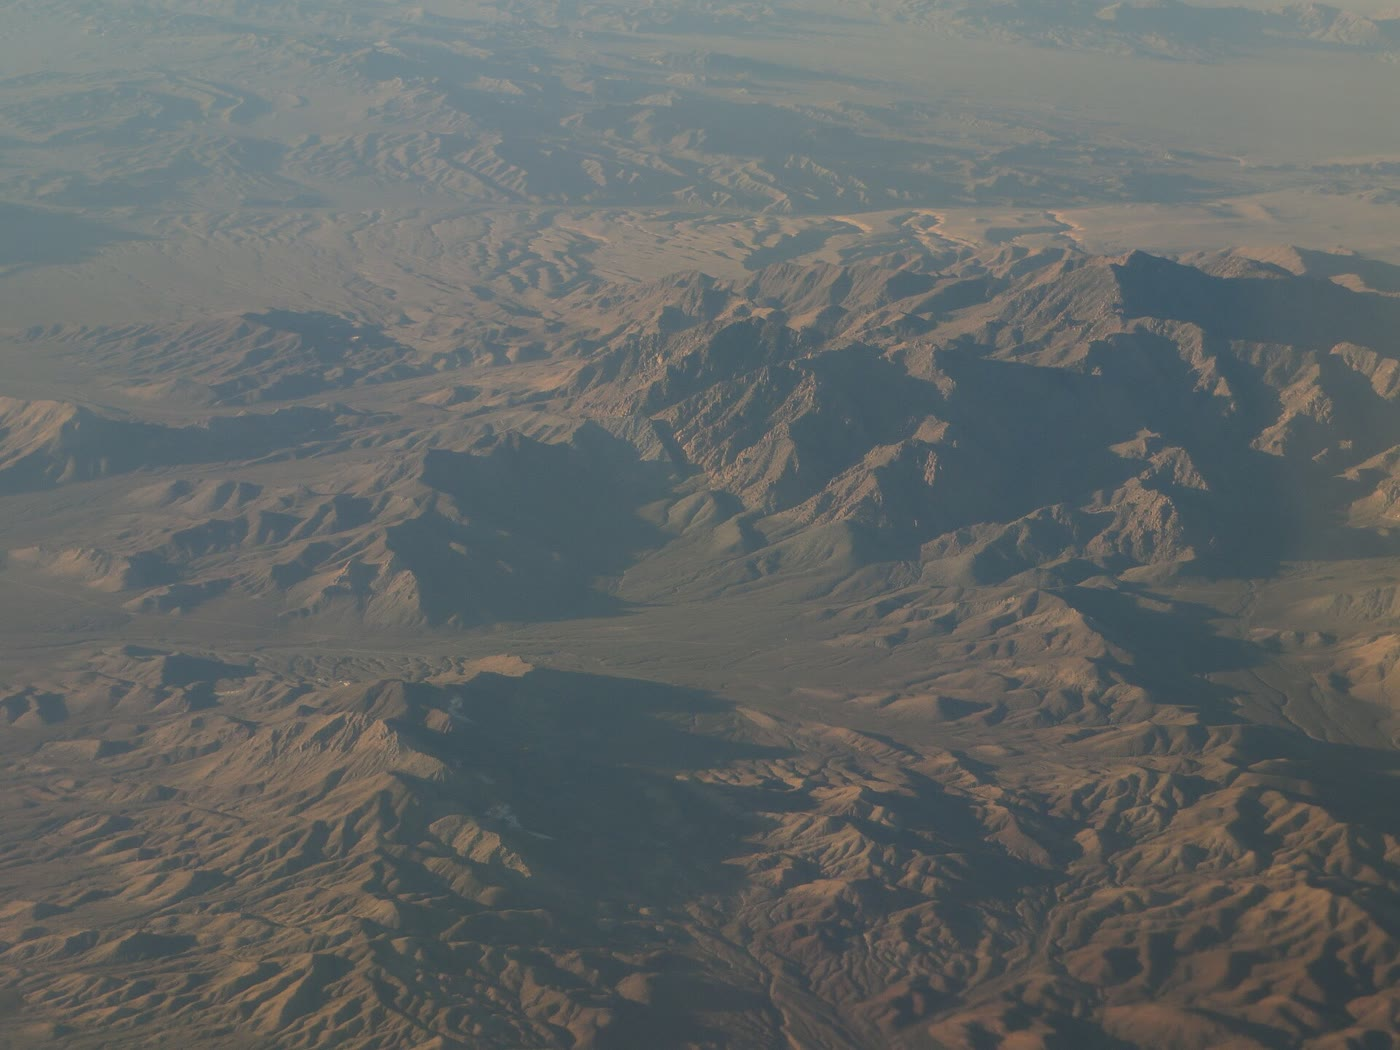
\includegraphics[width=\linewidth]{images/book5/b3-basin-and-range.jpg}

{\scriptsize Topografia de bacias e cordilheiras (\textit{basin and range}) ao sul de Death Valley, Califórnia,
vista aérea: serras paralelas de blocos de falha inclinados separados por
bacias preenchidas por sedimentos. Foto Ken Lund, CC BY-SA 2.0.}
\end{minipage}
\end{inthefield}
% ledger: photo:b3-basin-and-range

\section{Exercícios}

\begin{exercise}[$\star$]\label{exo:b3:extension-strike-slip:1}
Um domínio de blocos rígidos em dominó tem falhas que mergulham \ang{35}; elas se formaram a
\ang{50}. Calcule o mergulho das camadas e o fator de extensão.
\end{exercise}

\begin{exercise}[$\star$]\label{exo:b3:extension-strike-slip:2}
Diga se cada degrau abre uma bacia ou eleva uma crista: uma falha dextral
com degrau para a direita; uma falha dextral com degrau para a esquerda; uma falha
sinistral com degrau para a esquerda; uma falha sinistral com degrau para a direita.
\end{exercise}

\begin{exercise}[$\star$]\label{exo:b3:extension-strike-slip:3}
A falha transformante do Mar Morto deslocou-se \qty{105}{km} em cerca de \qty{20}{Myr}.
Calcule a taxa média, em \unit{mm/yr}, e compare-a com a taxa de \qty{6}{mm/yr}
usada para a bacia do Mar Morto.
\end{exercise}

\begin{exercise}[$\star$]\label{exo:b3:extension-strike-slip:4}
Na porção central da Basin and Range, \qty{235}{km} de extensão correspondem a
\qty{200}{\percent}. Calcule a largura da região antes e depois. Faça o
mesmo para a porção norte, a \qty{50}{\percent}.
\end{exercise}

\begin{exercise}[$\star\star$]\label{exo:b3:extension-strike-slip:5}
A falha de San Andreas deslocou-se pelo menos \qty{563}{km} em 15 a
\qty{20}{Myr}. Calcule a faixa das taxas médias e compare-as com uma
deriva atual de cerca de \qty{51}{mm/yr}. Explique o que poderia justificar a diferença.
\end{exercise}

\begin{exercise}[$\star\star$]\label{exo:b3:extension-strike-slip:6}
Com $\mu = 0.6$, calcule a razão $\sigma_1/\sigma_3$ necessária para fazer deslizar as falhas normais
que mergulham \ang{60}, \ang{50} e \ang{40}, e o mergulho de bloqueio.
\end{exercise}

\begin{exercise}[$\star\star$]\label{exo:b3:extension-strike-slip:7}
Calcule o mergulho de bloqueio de uma falha normal para $\mu = 0.4$ e $\mu = 0.2$.
Determine o coeficiente de atrito que permitiria que uma falha que mergulha \ang{15} deslize sob um
$\sigma_1$ vertical.
\end{exercise}

\begin{exercise}[$\star\star$]\label{exo:b3:extension-strike-slip:8}
Em uma seção sísmica paralela ao deslocamento, uma \omterm{def:b3:extension-strike-slip:detachment}{falha lístrica} tem afastamento horizontal de
\qty{2.5}{km}; ela se achata em um descolamento a \qty{4.0}{km} de profundidade. Calcule a
área da depressão abaixo do topo original do bloco superior e abaixo de uma camada
que primeiro aparece a \qty{1.5}{km} de profundidade.
\end{exercise}

\begin{exercise}[$\star\star$]\label{exo:b3:extension-strike-slip:9}
A bacia do Mar Morto tem \qty{132}{km} de comprimento e foi estirada pelo fator 1.19
ao longo de seu eixo. Calcule seu comprimento inicial e o estiramento, e o tempo
que o estiramento leva a \qty{6}{mm/yr}.
\end{exercise}

\begin{exercise}[$\star\star\star$]\label{exo:b3:extension-strike-slip:10}
Blocos separados por \qty{3.0}{km}, medidos perpendicularmente às suas falhas, giram
de mergulhos de falha de \ang{60} para \ang{45}. Calcule a largura horizontal de um
bloco antes e depois, a extensão por bloco e o mergulho das camadas.
Por que as camadas devem mergulhar no sentido oposto ao das falhas?
\end{exercise}

\begin{exercise}[$\star\star\star$]\label{exo:b3:extension-strike-slip:11}
Dê os ângulos dos cisalhamentos R e R$'$ e das fraturas de tração para uma
rocha com $\phi = \ang{40}$ em uma zona sinistral de direção L--O, em
azimutes, e seus sentidos de deslizamento.
\end{exercise}

\begin{exercise}[$\star\star\star$]\label{exo:b3:extension-strike-slip:12}
Forma-se um domínio de \omterm{def:b3:extension-strike-slip:domino}{falhamento em dominó} com as falhas no mergulho mais favorável ao
deslizamento, e o domínio gira até que elas travem. Calcule o maior fator de extensão que
a rotação, sozinha, produz para $\mu = 0.6$ e para $\mu = 0.85$, e diga quais
rochas podem ser estendidas ainda mais antes que novas falhas tenham de se formar.
\end{exercise}

\section{Problema: O semigráben de Merrow}

\begin{problem}[{Problema de fim de semana --- a extensão de uma borda de rifte inventada,
a partir de seus falhamentos em dominó, de sua falha lístrica, de seu complexo de núcleo
metamórfico e de sua falha de transferência}]
\label{pb:b3:extension-strike-slip:1}
% values: calc/ch09.py; domino_extension.py; rollover.py
O semigráben de Merrow é uma bacia inventada na borda de um rifte continental.
Sua falha principal é lístrica, com mergulho de \ang{60} na superfície. No seu
bloco superior, um domínio com \qty{24.0}{km} de largura é cortado por falhas planas, hoje
mergulhando \ang{42} para L, entre as quais as camadas mergulham \ang{18} para O. Em uma
seção sísmica paralela ao deslizamento, a falha principal tem afastamento horizontal de
\qty{3.2}{km}, e o topo de seu bloco superior afunda abaixo do nível original em uma área de
\qty{16.0}{km^2}. Ao longo da direção, para o sul, a erosão removeu a placa superior do mesmo
sistema e expôs um \omterm{def:b3:extension-strike-slip:core-complex}{complexo de núcleo metamórfico}. Para o norte, uma falha de transferência
sinistral liga o semigráben ao seguinte. Adote $\mu =
0.6$, $g = \qty{9.8}{m/s^2}$ e densidade crustal de
\qty{2800}{kg/m^3}.

\medskip\noindent\textbf{Parte I --- O falhamento em dominó.}
\begin{enumerate}
  \item Por que o mergulho inicial das falhas é a soma dos mergulhos atuais da falha e
        das camadas? Dê-o e compare-o com a teoria de Anderson.
  \item Calcule o fator de extensão do domínio.
  \item Calcule sua largura inicial e a extensão que ele registra.
  \item Calcule a razão $\sigma_1/\sigma_3$ necessária para fazer as falhas deslizarem agora,
        e compare-a com a de falhas novas, bem orientadas.
  \item Em que mergulho essas falhas travam, e que fator de extensão o domínio poderia
        atingir apenas por rotação? O que acontece então?
\end{enumerate}

\medskip\noindent\textbf{Parte II --- A falha principal lístrica.}
\begin{enumerate}[resume]
  \item Explique, com a construção de afastamento horizontal constante, por que as camadas do bloco
        superior se inclinam em direção à falha.
  \item Calcule a profundidade do descolamento.
  \item A área da depressão é conhecida com precisão de \qty{10}{\percent}. Com que
        precisão se conhece a profundidade?
  \item Qual área de depressão se prevê para uma camada que primeiro aparece a \qty{2.0}{km}
        de profundidade?
  \item Qual é a extensão horizontal através da falha principal?
  \item Como os sedimentos do semigráben registram a atividade da
        falha?
\end{enumerate}

\medskip\noindent\textbf{Parte III --- O complexo de núcleo metamórfico.}
\begin{enumerate}[resume]
  \item Os milonitos do bloco inferior entraram em equilíbrio a \qty{5.5}{kbar}. Calcule
        sua profundidade.
  \item Suas micas fecharam para o argônio a \qty{24}{Ma}, e seixos dos mesmos
        milonitos aparecem no preenchimento do semigráben a \qty{16}{Ma}. Calcule a
        taxa média de exumação, tomando a profundidade de fechamento como a profundidade da
        questão anterior.
  \item Para trazer os milonitos à superfície, quanto deslizamento é necessário em um descolamento
        de mergulho médio de \ang{30}, e quanta extensão horizontal?
  \item Hoje o descolamento mergulha \ang{15} na superfície. Poderia ele ter deslizado
        com esse mergulho sob um $\sigma_1$ vertical? Dê duas saídas.
  \item Se ele deslizou a \ang{45} em profundidade, de que ângulo a parte exposta
        girou, e por quê?
  \item Compare a extensão do \omterm{def:b3:extension-strike-slip:core-complex}{complexo de núcleo metamórfico} com a do
        semigráben.
\end{enumerate}

\medskip\noindent\textbf{Parte IV --- A falha de transferência.}
\begin{enumerate}[resume]
  \item A falha de transferência sinistral dá um degrau de \qty{4.0}{km} para a esquerda, com seus dois
        ramos sobrepostos ao longo de \qty{3.0}{km}. O degrau abre uma bacia
        ou eleva uma crista?
  \item A falha deslizou a \qty{5}{mm/yr} durante \qty{1.2}{Myr}. Calcule
        o deslocamento.
  \item Calcule a área aberta, o comprimento do assoalho da bacia (sobreposição mais
        deslocamento) e sua razão entre comprimento e largura.
  \item Compare essa razão com a da bacia do Mar Morto, com \qty{132}{km} de comprimento e largura de 7
        a \qty{10}{km} de largura.
  \item Onde a mesma falha se curva no sentido oposto, que estrutura se forma, e
        o que mostraria uma seção transversal que a atravesse?
  \item Qual é a extensão horizontal total através do semigráben de Merrow,
        a partir de sua falha principal e de seus \omterm{def:b3:extension-strike-slip:domino}{falhamentos em dominó}?
\end{enumerate}
\end{problem}
